%% abtex2-modelo-include-comandos.tex, v-1.9.5 laurocesar
%% Copyright 2012-2015 by abnTeX2 group at http://www.abntex.net.br/ 
%%
%% This work may be distributed and/or modified under the
%% conditions of the LaTeX Project Public License, either version 1.3
%% of this license or (at your option) any later version.
%% The latest version of this license is in
%%   http://www.latex-project.org/lppl.txt
%% and version 1.3 or later is part of all distributions of LaTeX
%% version 2005/12/01 or later.
%%
%% This work has the LPPL maintenance status `maintained'.
%% 
%% The Current Maintainer of this work is the abnTeX2 team, led
%% by Lauro César Araujo. Further information are available on 
%% http://www.abntex.net.br/
%%
%% This work consists of the files abntex2-modelo-include-comandos.tex
%% and abntex2-modelo-img-marca.pdf
%%

% ---
% Este capítulo, utilizado por diferentes exemplos do abnTeX2, ilustra o uso de
% comandos do abnTeX2 e de LaTeX.
% ---
 
\chapter{Greedy Heuristic Selection}\label{ghs}

\chapterprecis{The purpose of this section is to introduce the meta$-$reasoning proposed.}\index{sinopse de capítulo}

% ---
\section{Problem Formulation}
% ---
When solving $\triangledown$ using the consistent heuristic function $h_{max}(\zeta\sp{'})$ for $\zeta\sp{'} \subseteq \zeta$, A$\sp{*}$ expands in the worst case $J(\zeta\sp{'}, \triangledown)$ nodes, where

\begin{equation}
J(\zeta\sp{'},\triangledown) = |\{s \in V | f_{max}(s,\zeta\sp{'}) \leq C\sp{*}\}|
\label{eq:eq_size_search_tree_1}
\end{equation}

\begin{equation}
J(\zeta\sp{'},\triangledown) = |\{s \in V | h_{max}(s,\zeta\sp{'}) \leq C\sp{*} - g(s)\}|
\label{eq:eq_size_search_tree_2}
\end{equation}

We present a greedy algorithm for approximately solving the following optimization problem,

\begin{equation}
\begin{split}
\textbf{minimize}_{\zeta\sp{'} \in 2\sp{|\zeta|}}J(\zeta\sp{'}, \triangledown) \\
\textbf{subject to} |\zeta\sp{'} = N|
\end{split}
\end{equation}

Where $N$ could be determined by a hard constraint such as the maximum number of \texttt{PDBs} one can store in memory.

% ---
\section{GHS Algorithm}
% ---
\noindent
Algorithm \ref{alg:ghs_algorithm} presents Greedy Heuristic Selection (\texttt{GHS}), an approximation algorithm for selecting a subset $\zeta\sp{'} \subseteq \zeta$.

The algorithm receives as input a planning problem $\triangledown$, a set of heuristics $\zeta$, a cardinality size $N$, and it returns a subset $\zeta\sp{'} \subseteq \zeta$ of size $N$. In each iteration \texttt{GHS} greedily selects from $\zeta$ the heuristic $h$ which will result in the largest reduction of the value of $J$ (line 3). \texttt{GHS} returns $\zeta\sp{'}$ once it has the desired cardinality size $N$.\\

\begin{algorithm}[H]
 
\textbf{Input:} Problem $\triangledown$, set  of heuristics $\zeta$, cardinality $N$
 
\textbf{Ouput:} heuristic subset $\zeta\sp{'} \subseteq \zeta$ of size $N$
 
$\zeta\sp{'} \leftarrow \emptyset$
 
\While{$|\zeta\sp{'}| < N$ do} {
 
	$h \leftarrow \texttt{argmin}_{h \in \zeta} J(\zeta\sp{'} \cup \{h\}, \triangledown) $
 
	$\zeta\sp{'} \leftarrow \zeta\sp{'} \cup \{h\}$
 
	return $\zeta\sp{'}$
}
\caption{Greedy Heuristic Selection}
\label{alg:ghs_algorithm}
\end{algorithm}

\subsection{GHS Approximation Analysis}
In the following analysis all heuristic functions are assumed to be consistent. We also assume that A$\sp{*}$ expands all nodes $n$ with $f(n) \leq C\sp{*}$ while solving $\triangledown$, as shown in Equation \eqref{eq:eq_size_search_tree_1}.

\section{Stratified Sampling (SS)}
Stratified Sampling is a prediction algorithm that estimate the number of nodes expanded by some heuristic.\\

\cite{knuth1975Estimating} created a method to estimate the size of the search tree such as IDA$\sp{*}$. It works doing random walk from the root of the tree. Knuth's assumption is that all branches have the same structure. So, performing a random walk down one branch is enought to estimate the size of the search tree. However, the method does not work well for unbalanced search tree. \cite{chen1992heuristic}
 solved this problem with a stratification of the search tree through a \textit{type system} to reduce the variance of the sampling process\cite{lelis2013predicting}

In the figure \ref{fig:ss_ts} each node of the Search Space is mapped to the \textit{Type System}

\begin{figure}[htb]
\centering 
\begin{tikzpicture}

% -- center, xdim, ydim
\draw[very thick,cyan] \boundellipse{-2,0}{2}{4};
\draw[very thick,cyan] \boundellipse{6,0}{1}{2};
	
  % First, define nodes
% -- points F  
  
  \draw (-2,3) node[circle, inner sep=0.8pt, fill=cyan, label={below:{}}] (E) {};  
  \draw (6,1) node[circle, inner sep=0.8pt, fill=cyan, label={below:{}}] (F) {}; 

  \draw[very thick,cyan, ->>]  (E) .. controls +(5,-3) and +(-4,1).. (F);
  \path  ($(E)+(0,0.2)$) .. controls +(5,-3) and +(-4,1)..  ($(F)+(0,0.2)$) 
     {\foreach \i in {1,...,40} {  coordinate[pos=0.15+0.75*\i/40] (p\i) } };

  \draw (-1,2) node[circle, inner sep=0.8pt, fill=cyan, label={below:{}}] (A) {};
  \draw[very thick,cyan, ->>]  (A) .. controls +(5,-3) and +(-4,1).. (F);
  \path  ($(A)+(0,0.2)$) .. controls +(5,-3) and +(-4,1)..  ($(F)+(0,0.2)$) 
     {\foreach \i in {1,...,40} {  coordinate[pos=0.15+0.75*\i/40] (p\i) } };
	
  \draw (-3,0) node[circle, inner sep=0.8pt, fill=cyan, label={below:{}}] (B) {};
  \draw[very thick,cyan, ->>]  (B) .. controls +(5,-3) and +(-4,1).. (F);
  \path  ($(B)+(0,0.2)$) .. controls +(5,-3) and +(-4,1)..  ($(F)+(0,0.2)$) 
     {\foreach \i in {1,...,40} {  coordinate[pos=0.15+0.75*\i/40] (p\i) } };
	
% -- points in G

  \draw (-2,1) node[circle, inner sep=0.8pt, fill=cyan, label={below:{}}] (C) {};
  \draw (6.5,0) node[circle, inner sep=0.8pt, fill=cyan, label={below:{}}] (G) {};
  \draw[very thick,cyan, ->>]  (C) .. controls +(5,-3) and +(-4,1).. (G);
  \path  ($(C)+(0,0.2)$) .. controls +(5,-3) and +(-4,1)..  ($(G)+(0,0.2)$) 
     {\foreach \i in {1,...,40} {  coordinate[pos=0.15+0.75*\i/40] (p\i) } };	

\draw (-1,0) node[circle, inner sep=0.8pt, fill=cyan, label={below:{}}] (D) {};	
\draw[very thick,cyan, ->>]  (D) .. controls +(5,-3) and +(-4,1).. (G);
  \path  ($(C)+(0,0.2)$) .. controls +(5,-3) and +(-4,1)..  ($(G)+(0,0.2)$) 
     {\foreach \i in {1,...,40} {  coordinate[pos=0.15+0.75*\i/40] (p\i) } };	

\draw (-3,-1) node[circle, inner sep=0.8pt, fill=cyan, label={below:{}}] (H) {};	
\draw[very thick,cyan, ->>]  (H) .. controls +(5,-3) and +(-4,1).. (G);
  \path  ($(C)+(0,0.2)$) .. controls +(5,-3) and +(-4,1)..  ($(G)+(0,0.2)$) 
     {\foreach \i in {1,...,40} {  coordinate[pos=0.15+0.75*\i/40] (p\i) } };
	
% -- X
\draw (-2,-2) node[circle, inner sep=0.8pt, fill=cyan, label={below:{}}] (J) {};
  \draw (6,-1) node[circle, inner sep=0.8pt, fill=cyan, label={below:{}}] (X) {};
  \draw[very thick,cyan, ->>]  (J) .. controls +(5,-3) and +(-4,1).. (X);
  \path  ($(C)+(0,0.2)$) .. controls +(5,-3) and +(-4,1)..  ($(G)+(0,0.2)$) 
     {\foreach \i in {1,...,40} {  coordinate[pos=0.15+0.75*\i/40] (p\i) } };

\draw (-2,-3) node[circle, inner sep=0.8pt, fill=cyan, label={below:{}}] (K) {};
\draw[very thick,cyan, ->>]  (K) .. controls +(5,-3) and +(-4,1).. (X);
  \path  ($(C)+(0,0.2)$) .. controls +(5,-3) and +(-4,1)..  ($(G)+(0,0.2)$) 
     {\foreach \i in {1,...,40} {  coordinate[pos=0.15+0.75*\i/40] (p\i) } };

$\node [xshift=1cm,yshift=2cm] (A) at (-3,3) {Search Space};$

$\node [xshift=1cm,yshift=2cm] (A) at (5,1) {Type System};$
	
\end{tikzpicture}
\caption{Type system and the Search Space Representation.} \label{fig:ss_ts}
\end{figure}


\subsection{Type System}
The \textit{Type System} is a partition of the states in the state space. It is calculated based of any property of each node in the search tree. \cite{Lelis2013CC}

A common misconception is think of \textit{type system} as state$-$space abstractions. \cite{Prieditis93} defines a state$-$space abstraction as a simplified version of the problem in which:
\begin{itemize}
\item The cost of the least$-$cost path between two abstracted states must less than or equal to the cost of the least$-$cost path between the corresponding two states in the original state$-$space.
\item Goal states in the original state$-$space must be goal states in the abstracted state$-$space.
\end{itemize}

In contrast with state$-$space abstractions, a \textit{type system} does not have these two requeriments. A \textit{type system} is just a partition of the nodes in the search tree.

The \textit{type system} can not be represented as a graph since \textit{type system} does not necessarily define relation between the types.

The relation between \textit{type system} and abstractions is the following: The \textit{type system} can not necessarily be used as abstractions, abstractions can always be used as \textit{type system}.








\theoremstyle{definition}
\begin{definition}{Type System}

\end{definition}


\begin{figure}[htb]
\centering
\begin{forest}
 [\usebox\myboxc \hspace*{1.4in} \usebox\myboxb]
\end{forest}
\caption{The heuristic value is the position of the empty space in a Specific state.} \label{fig:type_system}
\end{figure}

% print types

\begin{forest}
 [\usebox\myboxcenter]
 $\node [xshift=1cm,yshift=2cm] (A) at (2,0) {(2, M)};$
\end{forest}

\begin{forest}
 [\usebox\myboxcornerone]
 $\node [xshift=1cm,yshift=2cm] (A) at (2,0) {(4, C)};$
\end{forest}

\begin{forest}
 [\usebox\myboxmediumleft \hspace*{0.2in} \usebox\myboxmediumup]
 $\node [xshift=1cm,yshift=2cm] (A) at (4,0) {(3, E)};$
\end{forest}

\begin{forest}
 [\usebox\myboxcornerthree \hspace*{0.2in} \usebox\myboxcornertwo]
 $\node [xshift=1cm,yshift=2cm] (A) at (4,0) {(2, C)};$
\end{forest}


\begin{forest}
 [\usebox\myboxmediumdown \hspace*{0.2in} \usebox\myboxmediumright]
 $\node [xshift=1cm,yshift=2cm] (A) at (4,0) {(1, E)};$
\end{forest}


\begin{forest}
 [\usebox\myboxcornerfour]
 $\node [xshift=1cm,yshift=2cm] (A) at (2,0) {(0, C)};$
\end{forest}

% -- Explaining Stratified Sampling
In the Figure \ref{fig:ts_search_tree}, we can see how \textit{Type System} works. In the Level 1, we have the root node, we add the property called weight or (\textit{W}) initialized with one. Let's suppose that three nodes are generated by the root node in the Level 2. The nodes in the Level 2 have the following types: red, blue and red respectively, and each node recive the same \textit{W} of the father. In the Level 2 we apply the concept of \textit{Type System}, two states in the same level that have the same type (The same color) root subtrees  of the same type and only one state per state must be explored. There are two nodes with type red in Level 2. So, we choose randomly one of them. Let's suppose we choose the right red node. Then, we have to update the number of nodes with the type red using the \textit{W}, both red node types have \textit{W = 1}, then we sum the \textit{W} and the the new \textit{W = 2}. So, in the Level 2 we will have two nodes of red type and one node with blue type. \\

When nodes in the Level 2 are expanded. The blue node expands one node of type blue and the red node expands two nodes of type red and blue. The question here is how many nodes would be generated in the Level 3? The answer is: $1 \times \textcolor{cyan}{blue} + 2 \times \textcolor{red}{red} + 2 \times \textcolor{cyan}{blue}$. So, in the Level 3 we will have 2 nodes of red type and 3 nodes of type blue. \\ 

In the Level 3 the \textit{W} of the node blue would be the same \textit{W} of the father. The father has the \textit{W = 1}, then the child has the \textit{W = 1}. The \textit{W} of the red type and blue type would be 2. Once the \textit{W} has been updated for each node in the Level 3 we apply the concept of \textit{Type System} again. There are two nodes with type blue. So, we choose randomly one of them and update the \textit{W}. Let's choose the right blue type and the updated \textit{W} would be 3 because 1 from the left blue type plus the 2 from the right blue type. \\

When nodes in the Level 3 are expanded. The red node expands two nodes of types red and blue and the blue node expands one of the red. How many nodes would be generated at Level 4? The answer is: $2 \times \textcolor{red}{red} + 3 \times \textcolor{red}{red} + 2 \times \textcolor{cyan}{blue}$. So, in the Level 4 we will have five nodes of type red and two nodes of type blue.\\

The number of nodes expanded in the search tree is obtained summing all \textit{W} plus one (The root node). So, the number of nodes expanded in the search tree would be $ 15 + 1 = 16$. \\

\begin{figure}[htb]
\centering
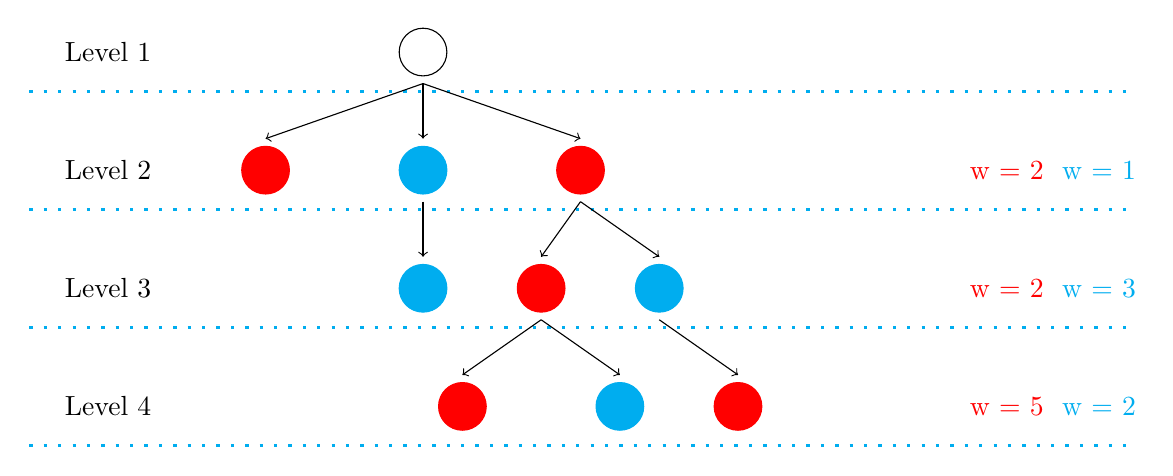
\begin{tikzpicture}

\draw[very thick,cyan,loosely dotted] (-2,0) -- (12,0);
\draw[very thick,cyan,loosely dotted] (-2,-1.5) -- (12,-1.5);
\draw[very thick,cyan,loosely dotted] (-2,-3) -- (12,-3);
\draw[very thick,cyan,loosely dotted] (-2,-4.5) -- (12,-4.5);

\node [xshift=1cm,yshift=2cm] (A) at (-2,-1.5) {Level 1};
\node [xshift=1cm,yshift=2cm] (A) at (-2,-3) {Level 2};
\node [xshift=1cm,yshift=2cm] (A) at (-2,-4.5) {Level 3};
\node [xshift=1cm,yshift=2cm] (A) at (-2,-6) {Level 4};

% -- level 1
\draw[black,fill=white] (3,0.5) circle (2ex);

% -- level 2
\draw[red,fill=red] (1,-1) circle (2ex);
\draw[cyan,fill=cyan] (3,-1) circle (2ex);
\draw[red,fill=red] (5,-1) circle (2ex);

% -- level 3
\draw[cyan,fill=cyan] (3,-2.5) circle (2ex);
\draw[red,fill=red] (4.5,-2.5) circle (2ex);
\draw[cyan,fill=cyan] (6,-2.5) circle (2ex);

% -- level 4
\draw[red,fill=red] (3.5,-4) circle (2ex);
\draw[cyan,fill=cyan] (5.5,-4) circle (2ex);
\draw[red,fill=red] (7,-4) circle (2ex);

% -- draw arrows
\draw[->] (3,0.1) -- (1,-0.6);
\draw[->] (3,0.1) -- (3,-0.6);
\draw[->] (3,0.1) -- (5,-0.6);

\draw[->] (3,-1.4) -- (3,-2.1);

\draw[->] (5,-1.4) -- (4.5,-2.1);
\draw[->] (5,-1.4) -- (6,-2.1);

\draw[->] (4.5,-2.9) -- (3.5,-3.6);
\draw[->] (4.5,-2.9) -- (5.5,-3.6);

\draw[->] (6,-2.9) -- (7,-3.6);

\node [xshift=1cm,yshift=2cm] (A) at (10,-3) {\textcolor{red}{w = 2 } \textcolor{cyan}{w = 1}};
\node [xshift=1cm,yshift=2cm] (A) at (10,-4.5) {\textcolor{red}{w = 2 } \textcolor{cyan}{w = 3}};
\node [xshift=1cm,yshift=2cm] (A) at (10,-6) {\textcolor{red}{w = 5 } \textcolor{cyan}{w = 2}};
\end{tikzpicture}
\caption{Search tree using Type System} \label{fig:ts_search_tree}
\end{figure}

\section{Modeling}
The resources of how to run the experiments.



\clearpage